% Created by tikzDevice version 0.12.6 on 2025-04-23 11:51:08
% !TEX encoding = UTF-8 Unicode
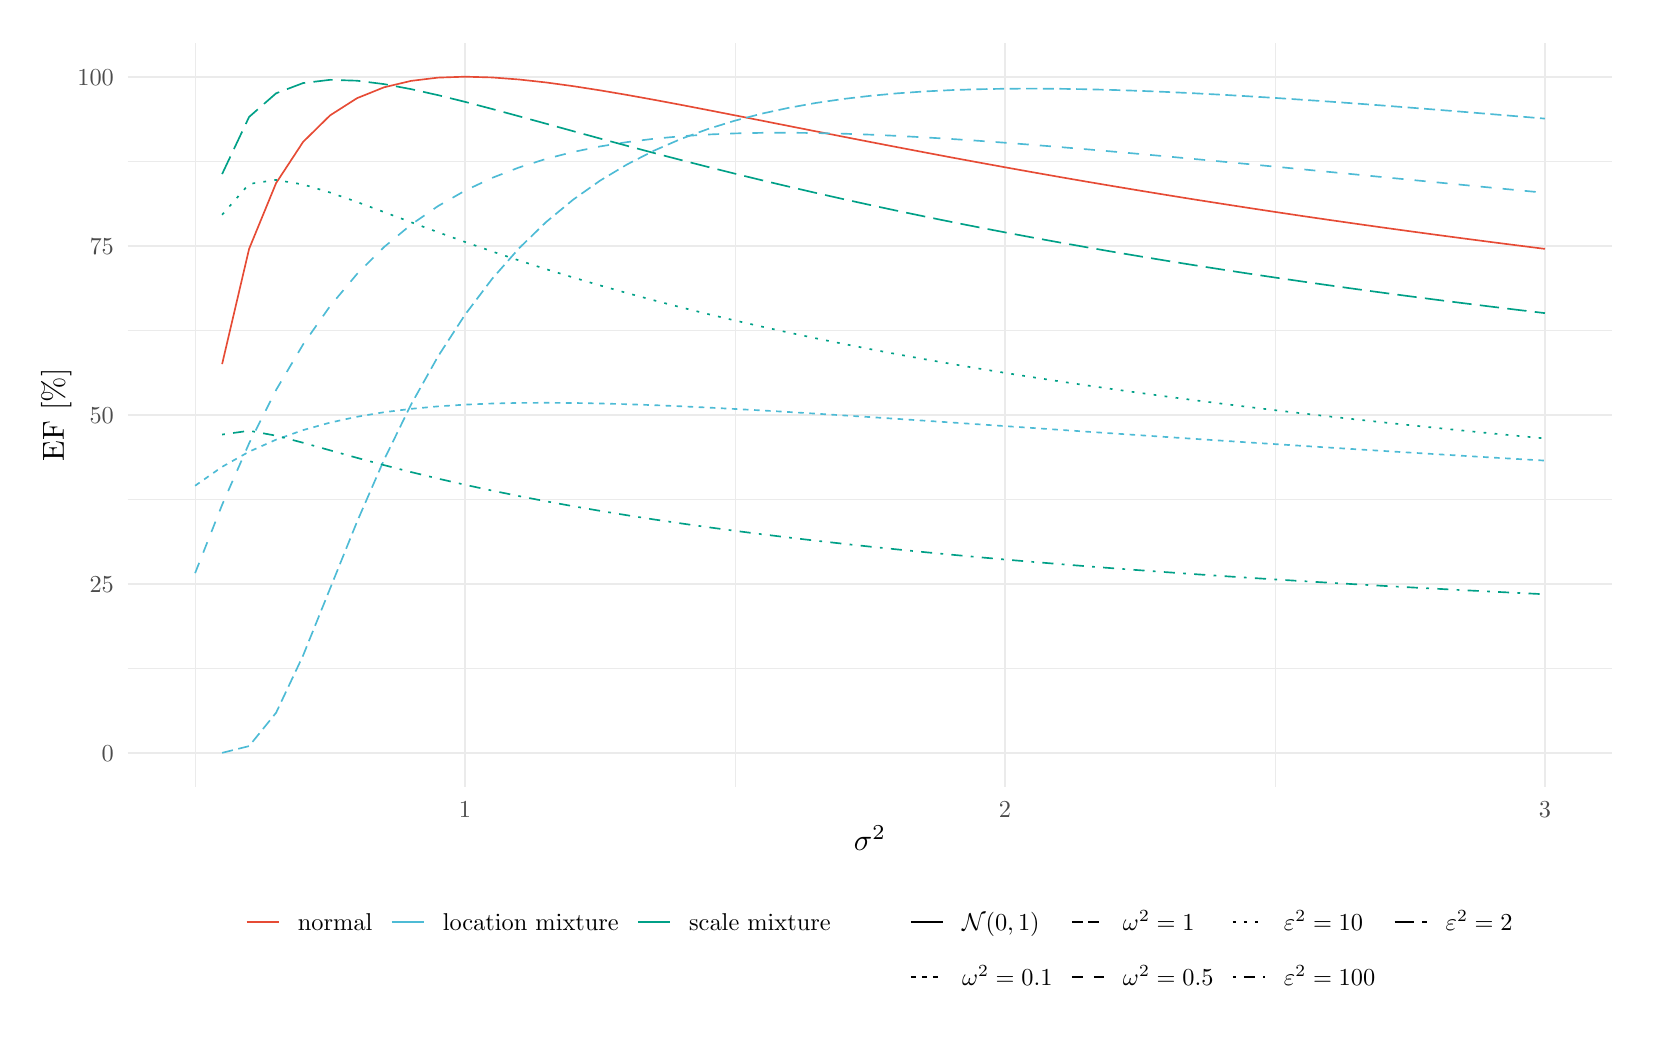
\begin{tikzpicture}[x=1pt,y=1pt]
\definecolor{fillColor}{RGB}{255,255,255}
\path[use as bounding box,fill=fillColor,fill opacity=0.00] (0,0) rectangle (578.16,361.35);
\begin{scope}
\path[clip] ( 36.11, 87.09) rectangle (572.66,355.85);
\definecolor{drawColor}{gray}{0.92}

\path[draw=drawColor,line width= 0.3pt,line join=round] ( 36.11,129.84) --
	(572.66,129.84);

\path[draw=drawColor,line width= 0.3pt,line join=round] ( 36.11,190.92) --
	(572.66,190.92);

\path[draw=drawColor,line width= 0.3pt,line join=round] ( 36.11,252.01) --
	(572.66,252.01);

\path[draw=drawColor,line width= 0.3pt,line join=round] ( 36.11,313.09) --
	(572.66,313.09);

\path[draw=drawColor,line width= 0.3pt,line join=round] ( 60.50, 87.09) --
	( 60.50,355.85);

\path[draw=drawColor,line width= 0.3pt,line join=round] (255.61, 87.09) --
	(255.61,355.85);

\path[draw=drawColor,line width= 0.3pt,line join=round] (450.72, 87.09) --
	(450.72,355.85);

\path[draw=drawColor,line width= 0.6pt,line join=round] ( 36.11, 99.30) --
	(572.66, 99.30);

\path[draw=drawColor,line width= 0.6pt,line join=round] ( 36.11,160.38) --
	(572.66,160.38);

\path[draw=drawColor,line width= 0.6pt,line join=round] ( 36.11,221.47) --
	(572.66,221.47);

\path[draw=drawColor,line width= 0.6pt,line join=round] ( 36.11,282.55) --
	(572.66,282.55);

\path[draw=drawColor,line width= 0.6pt,line join=round] ( 36.11,343.63) --
	(572.66,343.63);

\path[draw=drawColor,line width= 0.6pt,line join=round] (158.05, 87.09) --
	(158.05,355.85);

\path[draw=drawColor,line width= 0.6pt,line join=round] (353.16, 87.09) --
	(353.16,355.85);

\path[draw=drawColor,line width= 0.6pt,line join=round] (548.27, 87.09) --
	(548.27,355.85);
\definecolor{drawColor}{RGB}{230,75,53}

\path[draw=drawColor,line width= 0.6pt,line join=round] ( 70.26,239.78) --
	( 80.01,281.41) --
	( 89.77,305.19) --
	( 99.52,320.06) --
	(109.28,329.66) --
	(119.03,335.88) --
	(128.79,339.80) --
	(138.54,342.12) --
	(148.30,343.30) --
	(158.05,343.63) --
	(167.81,343.36) --
	(177.56,342.62) --
	(187.32,341.55) --
	(197.08,340.22) --
	(206.83,338.70) --
	(216.59,337.04) --
	(226.34,335.28) --
	(236.10,333.45) --
	(245.85,331.57) --
	(255.61,329.66) --
	(265.36,327.73) --
	(275.12,325.80) --
	(284.87,323.88) --
	(294.63,321.96) --
	(304.39,320.06) --
	(314.14,318.18) --
	(323.90,316.32) --
	(333.65,314.48) --
	(343.41,312.68) --
	(353.16,310.90) --
	(362.92,309.15) --
	(372.67,307.43) --
	(382.43,305.74) --
	(392.18,304.09) --
	(401.94,302.46) --
	(411.70,300.86) --
	(421.45,299.29) --
	(431.21,297.76) --
	(440.96,296.25) --
	(450.72,294.77) --
	(460.47,293.31) --
	(470.23,291.89) --
	(479.98,290.49) --
	(489.74,289.12) --
	(499.49,287.78) --
	(509.25,286.46) --
	(519.01,285.16) --
	(528.76,283.89) --
	(538.52,282.64) --
	(548.27,281.41);
\definecolor{drawColor}{RGB}{77,187,213}

\path[draw=drawColor,line width= 0.6pt,dash pattern=on 2pt off 2pt ,line join=round] ( 60.50,195.82) --
	( 70.26,202.66) --
	( 80.01,208.13) --
	( 89.77,212.48) --
	( 99.52,215.93) --
	(109.28,218.64) --
	(119.03,220.76) --
	(128.79,222.39) --
	(138.54,223.61) --
	(148.30,224.51) --
	(158.05,225.13) --
	(167.81,225.53) --
	(177.56,225.75) --
	(187.32,225.80) --
	(197.08,225.73) --
	(206.83,225.55) --
	(216.59,225.28) --
	(226.34,224.94) --
	(236.10,224.53) --
	(245.85,224.07) --
	(255.61,223.56) --
	(265.36,223.03) --
	(275.12,222.46) --
	(284.87,221.87) --
	(294.63,221.25) --
	(304.39,220.63) --
	(314.14,219.99) --
	(323.90,219.34) --
	(333.65,218.69) --
	(343.41,218.03) --
	(353.16,217.37) --
	(362.92,216.71) --
	(372.67,216.05) --
	(382.43,215.38) --
	(392.18,214.73) --
	(401.94,214.07) --
	(411.70,213.42) --
	(421.45,212.77) --
	(431.21,212.13) --
	(440.96,211.49) --
	(450.72,210.86) --
	(460.47,210.24) --
	(470.23,209.62) --
	(479.98,209.01) --
	(489.74,208.40) --
	(499.49,207.80) --
	(509.25,207.21) --
	(519.01,206.62) --
	(528.76,206.04) --
	(538.52,205.47) --
	(548.27,204.91);

\path[draw=drawColor,line width= 0.6pt,dash pattern=on 4pt off 2pt ,line join=round] ( 70.26, 99.31) --
	( 80.01,101.75) --
	( 89.77,113.80) --
	( 99.52,134.48) --
	(109.28,158.69) --
	(119.03,182.86) --
	(128.79,205.23) --
	(138.54,225.17) --
	(148.30,242.59) --
	(158.05,257.64) --
	(167.81,270.57) --
	(177.56,281.64) --
	(187.32,291.10) --
	(197.08,299.18) --
	(206.83,306.07) --
	(216.59,311.93) --
	(226.34,316.92) --
	(236.10,321.16) --
	(245.85,324.74) --
	(255.61,327.76) --
	(265.36,330.30) --
	(275.12,332.41) --
	(284.87,334.15) --
	(294.63,335.57) --
	(304.39,336.71) --
	(314.14,337.61) --
	(323.90,338.29) --
	(333.65,338.78) --
	(343.41,339.10) --
	(353.16,339.28) --
	(362.92,339.33) --
	(372.67,339.26) --
	(382.43,339.10) --
	(392.18,338.84) --
	(401.94,338.51) --
	(411.70,338.11) --
	(421.45,337.64) --
	(431.21,337.13) --
	(440.96,336.56) --
	(450.72,335.96) --
	(460.47,335.31) --
	(470.23,334.64) --
	(479.98,333.94) --
	(489.74,333.21) --
	(499.49,332.46) --
	(509.25,331.69) --
	(519.01,330.91) --
	(528.76,330.11) --
	(538.52,329.30) --
	(548.27,328.48);

\path[draw=drawColor,line width= 0.6pt,dash pattern=on 4pt off 4pt ,line join=round] ( 60.50,164.24) --
	( 70.26,188.92) --
	( 80.01,211.14) --
	( 89.77,230.44) --
	( 99.52,246.88) --
	(109.28,260.75) --
	(119.03,272.37) --
	(128.79,282.08) --
	(138.54,290.17) --
	(148.30,296.89) --
	(158.05,302.46) --
	(167.81,307.06) --
	(177.56,310.84) --
	(187.32,313.93) --
	(197.08,316.43) --
	(206.83,318.43) --
	(216.59,320.00) --
	(226.34,321.21) --
	(236.10,322.11) --
	(245.85,322.74) --
	(255.61,323.14) --
	(265.36,323.35) --
	(275.12,323.39) --
	(284.87,323.27) --
	(294.63,323.04) --
	(304.39,322.69) --
	(314.14,322.25) --
	(323.90,321.72) --
	(333.65,321.13) --
	(343.41,320.48) --
	(353.16,319.77) --
	(362.92,319.02) --
	(372.67,318.23) --
	(382.43,317.42) --
	(392.18,316.57) --
	(401.94,315.70) --
	(411.70,314.81) --
	(421.45,313.90) --
	(431.21,312.99) --
	(440.96,312.06) --
	(450.72,311.12) --
	(460.47,310.18) --
	(470.23,309.23) --
	(479.98,308.29) --
	(489.74,307.34) --
	(499.49,306.39) --
	(509.25,305.44) --
	(519.01,304.49) --
	(528.76,303.55) --
	(538.52,302.61) --
	(548.27,301.68);
\definecolor{drawColor}{RGB}{0,160,135}

\path[draw=drawColor,line width= 0.6pt,dash pattern=on 1pt off 3pt ,line join=round] ( 70.26,293.74) --
	( 80.01,304.87) --
	( 89.77,306.33) --
	( 99.52,304.68) --
	(109.28,301.78) --
	(119.03,298.35) --
	(128.79,294.71) --
	(138.54,291.04) --
	(148.30,287.43) --
	(158.05,283.91) --
	(167.81,280.50) --
	(177.56,277.23) --
	(187.32,274.09) --
	(197.08,271.09) --
	(206.83,268.21) --
	(216.59,265.45) --
	(226.34,262.81) --
	(236.10,260.28) --
	(245.85,257.85) --
	(255.61,255.53) --
	(265.36,253.30) --
	(275.12,251.15) --
	(284.87,249.09) --
	(294.63,247.11) --
	(304.39,245.20) --
	(314.14,243.35) --
	(323.90,241.58) --
	(333.65,239.87) --
	(343.41,238.21) --
	(353.16,236.61) --
	(362.92,235.07) --
	(372.67,233.57) --
	(382.43,232.12) --
	(392.18,230.72) --
	(401.94,229.36) --
	(411.70,228.04) --
	(421.45,226.75) --
	(431.21,225.51) --
	(440.96,224.30) --
	(450.72,223.12) --
	(460.47,221.98) --
	(470.23,220.87) --
	(479.98,219.78) --
	(489.74,218.73) --
	(499.49,217.70) --
	(509.25,216.70) --
	(519.01,215.72) --
	(528.76,214.76) --
	(538.52,213.83) --
	(548.27,212.92);

\path[draw=drawColor,line width= 0.6pt,dash pattern=on 1pt off 3pt on 4pt off 3pt ,line join=round] ( 70.26,214.32) --
	( 80.01,215.70) --
	( 89.77,213.92) --
	( 99.52,211.36) --
	(109.28,208.62) --
	(119.03,205.90) --
	(128.79,203.27) --
	(138.54,200.77) --
	(148.30,198.40) --
	(158.05,196.17) --
	(167.81,194.07) --
	(177.56,192.08) --
	(187.32,190.20) --
	(197.08,188.43) --
	(206.83,186.75) --
	(216.59,185.16) --
	(226.34,183.64) --
	(236.10,182.21) --
	(245.85,180.84) --
	(255.61,179.53) --
	(265.36,178.29) --
	(275.12,177.10) --
	(284.87,175.96) --
	(294.63,174.87) --
	(304.39,173.82) --
	(314.14,172.82) --
	(323.90,171.85) --
	(333.65,170.92) --
	(343.41,170.03) --
	(353.16,169.16) --
	(362.92,168.33) --
	(372.67,167.53) --
	(382.43,166.75) --
	(392.18,166.00) --
	(401.94,165.28) --
	(411.70,164.57) --
	(421.45,163.89) --
	(431.21,163.23) --
	(440.96,162.59) --
	(450.72,161.97) --
	(460.47,161.37) --
	(470.23,160.78) --
	(479.98,160.21) --
	(489.74,159.65) --
	(499.49,159.11) --
	(509.25,158.59) --
	(519.01,158.07) --
	(528.76,157.58) --
	(538.52,157.09) --
	(548.27,156.61);

\path[draw=drawColor,line width= 0.6pt,dash pattern=on 7pt off 3pt ,line join=round] ( 70.26,308.45) --
	( 80.01,329.09) --
	( 89.77,337.63) --
	( 99.52,341.33) --
	(109.28,342.50) --
	(119.03,342.18) --
	(128.79,340.95) --
	(138.54,339.14) --
	(148.30,336.96) --
	(158.05,334.54) --
	(167.81,331.97) --
	(177.56,329.33) --
	(187.32,326.65) --
	(197.08,323.96) --
	(206.83,321.29) --
	(216.59,318.65) --
	(226.34,316.05) --
	(236.10,313.51) --
	(245.85,311.01) --
	(255.61,308.58) --
	(265.36,306.20) --
	(275.12,303.88) --
	(284.87,301.62) --
	(294.63,299.42) --
	(304.39,297.28) --
	(314.14,295.19) --
	(323.90,293.16) --
	(333.65,291.18) --
	(343.41,289.25) --
	(353.16,287.38) --
	(362.92,285.55) --
	(372.67,283.77) --
	(382.43,282.04) --
	(392.18,280.35) --
	(401.94,278.71) --
	(411.70,277.10) --
	(421.45,275.53) --
	(431.21,274.01) --
	(440.96,272.51) --
	(450.72,271.06) --
	(460.47,269.64) --
	(470.23,268.25) --
	(479.98,266.89) --
	(489.74,265.56) --
	(499.49,264.27) --
	(509.25,263.00) --
	(519.01,261.76) --
	(528.76,260.55) --
	(538.52,259.36) --
	(548.27,258.20);
\end{scope}
\begin{scope}
\path[clip] (  0.00,  0.00) rectangle (578.16,361.35);
\definecolor{drawColor}{gray}{0.30}

\node[text=drawColor,anchor=base east,inner sep=0pt, outer sep=0pt, scale=  0.88] at ( 31.16, 96.27) {0};

\node[text=drawColor,anchor=base east,inner sep=0pt, outer sep=0pt, scale=  0.88] at ( 31.16,157.35) {25};

\node[text=drawColor,anchor=base east,inner sep=0pt, outer sep=0pt, scale=  0.88] at ( 31.16,218.44) {50};

\node[text=drawColor,anchor=base east,inner sep=0pt, outer sep=0pt, scale=  0.88] at ( 31.16,279.52) {75};

\node[text=drawColor,anchor=base east,inner sep=0pt, outer sep=0pt, scale=  0.88] at ( 31.16,340.60) {100};
\end{scope}
\begin{scope}
\path[clip] (  0.00,  0.00) rectangle (578.16,361.35);
\definecolor{drawColor}{gray}{0.30}

\node[text=drawColor,anchor=base,inner sep=0pt, outer sep=0pt, scale=  0.88] at (158.05, 76.08) {1};

\node[text=drawColor,anchor=base,inner sep=0pt, outer sep=0pt, scale=  0.88] at (353.16, 76.08) {2};

\node[text=drawColor,anchor=base,inner sep=0pt, outer sep=0pt, scale=  0.88] at (548.27, 76.08) {3};
\end{scope}
\begin{scope}
\path[clip] (  0.00,  0.00) rectangle (578.16,361.35);
\definecolor{drawColor}{RGB}{0,0,0}

\node[text=drawColor,anchor=base,inner sep=0pt, outer sep=0pt, scale=  1.10] at (304.39, 64.05) {$\sigma^2$};
\end{scope}
\begin{scope}
\path[clip] (  0.00,  0.00) rectangle (578.16,361.35);
\definecolor{drawColor}{RGB}{0,0,0}

\node[text=drawColor,rotate= 90.00,anchor=base,inner sep=0pt, outer sep=0pt, scale=  1.10] at ( 13.08,221.47) {EF [\%]};
\end{scope}
\begin{scope}
\path[clip] (  0.00,  0.00) rectangle (578.16,361.35);
\definecolor{drawColor}{RGB}{230,75,53}

\path[draw=drawColor,line width= 0.6pt,line join=round] ( 79.13, 38.18) -- ( 90.69, 38.18);
\end{scope}
\begin{scope}
\path[clip] (  0.00,  0.00) rectangle (578.16,361.35);
\definecolor{drawColor}{RGB}{77,187,213}

\path[draw=drawColor,line width= 0.6pt,line join=round] (131.49, 38.18) -- (143.05, 38.18);
\end{scope}
\begin{scope}
\path[clip] (  0.00,  0.00) rectangle (578.16,361.35);
\definecolor{drawColor}{RGB}{0,160,135}

\path[draw=drawColor,line width= 0.6pt,line join=round] (220.51, 38.18) -- (232.07, 38.18);
\end{scope}
\begin{scope}
\path[clip] (  0.00,  0.00) rectangle (578.16,361.35);
\definecolor{drawColor}{RGB}{0,0,0}

\node[text=drawColor,anchor=base west,inner sep=0pt, outer sep=0pt, scale=  0.88] at ( 97.64, 35.15) {normal};
\end{scope}
\begin{scope}
\path[clip] (  0.00,  0.00) rectangle (578.16,361.35);
\definecolor{drawColor}{RGB}{0,0,0}

\node[text=drawColor,anchor=base west,inner sep=0pt, outer sep=0pt, scale=  0.88] at (150.00, 35.15) {location mixture};
\end{scope}
\begin{scope}
\path[clip] (  0.00,  0.00) rectangle (578.16,361.35);
\definecolor{drawColor}{RGB}{0,0,0}

\node[text=drawColor,anchor=base west,inner sep=0pt, outer sep=0pt, scale=  0.88] at (239.02, 35.15) {scale mixture};
\end{scope}
\begin{scope}
\path[clip] (  0.00,  0.00) rectangle (578.16,361.35);
\definecolor{drawColor}{RGB}{0,0,0}

\path[draw=drawColor,line width= 0.6pt,line join=round] (319.11, 38.18) -- (330.67, 38.18);
\end{scope}
\begin{scope}
\path[clip] (  0.00,  0.00) rectangle (578.16,361.35);
\definecolor{drawColor}{RGB}{0,0,0}

\path[draw=drawColor,line width= 0.6pt,dash pattern=on 2pt off 2pt ,line join=round] (319.11, 18.23) -- (330.67, 18.23);
\end{scope}
\begin{scope}
\path[clip] (  0.00,  0.00) rectangle (578.16,361.35);
\definecolor{drawColor}{RGB}{0,0,0}

\path[draw=drawColor,line width= 0.6pt,dash pattern=on 4pt off 2pt ,line join=round] (377.28, 38.18) -- (388.85, 38.18);
\end{scope}
\begin{scope}
\path[clip] (  0.00,  0.00) rectangle (578.16,361.35);
\definecolor{drawColor}{RGB}{0,0,0}

\path[draw=drawColor,line width= 0.6pt,dash pattern=on 4pt off 4pt ,line join=round] (377.28, 18.23) -- (388.85, 18.23);
\end{scope}
\begin{scope}
\path[clip] (  0.00,  0.00) rectangle (578.16,361.35);
\definecolor{drawColor}{RGB}{0,0,0}

\path[draw=drawColor,line width= 0.6pt,dash pattern=on 1pt off 3pt ,line join=round] (435.46, 38.18) -- (447.02, 38.18);
\end{scope}
\begin{scope}
\path[clip] (  0.00,  0.00) rectangle (578.16,361.35);
\definecolor{drawColor}{RGB}{0,0,0}

\path[draw=drawColor,line width= 0.6pt,dash pattern=on 1pt off 3pt on 4pt off 3pt ,line join=round] (435.46, 18.23) -- (447.02, 18.23);
\end{scope}
\begin{scope}
\path[clip] (  0.00,  0.00) rectangle (578.16,361.35);
\definecolor{drawColor}{RGB}{0,0,0}

\path[draw=drawColor,line width= 0.6pt,dash pattern=on 7pt off 3pt ,line join=round] (493.90, 38.18) -- (505.46, 38.18);
\end{scope}
\begin{scope}
\path[clip] (  0.00,  0.00) rectangle (578.16,361.35);
\definecolor{drawColor}{RGB}{0,0,0}

\node[text=drawColor,anchor=base west,inner sep=0pt, outer sep=0pt, scale=  0.88] at (337.62, 35.15) {$\mathcal N (0, 1)$};
\end{scope}
\begin{scope}
\path[clip] (  0.00,  0.00) rectangle (578.16,361.35);
\definecolor{drawColor}{RGB}{0,0,0}

\node[text=drawColor,anchor=base west,inner sep=0pt, outer sep=0pt, scale=  0.88] at (337.62, 15.20) {$\omega^2 = 0.1$};
\end{scope}
\begin{scope}
\path[clip] (  0.00,  0.00) rectangle (578.16,361.35);
\definecolor{drawColor}{RGB}{0,0,0}

\node[text=drawColor,anchor=base west,inner sep=0pt, outer sep=0pt, scale=  0.88] at (395.79, 35.15) {$\omega^2 = 1$};
\end{scope}
\begin{scope}
\path[clip] (  0.00,  0.00) rectangle (578.16,361.35);
\definecolor{drawColor}{RGB}{0,0,0}

\node[text=drawColor,anchor=base west,inner sep=0pt, outer sep=0pt, scale=  0.88] at (395.79, 15.20) {$\omega^2= 0.5$};
\end{scope}
\begin{scope}
\path[clip] (  0.00,  0.00) rectangle (578.16,361.35);
\definecolor{drawColor}{RGB}{0,0,0}

\node[text=drawColor,anchor=base west,inner sep=0pt, outer sep=0pt, scale=  0.88] at (453.97, 35.15) {$\varepsilon^2 = 10$};
\end{scope}
\begin{scope}
\path[clip] (  0.00,  0.00) rectangle (578.16,361.35);
\definecolor{drawColor}{RGB}{0,0,0}

\node[text=drawColor,anchor=base west,inner sep=0pt, outer sep=0pt, scale=  0.88] at (453.97, 15.20) {$\varepsilon^2 = 100$};
\end{scope}
\begin{scope}
\path[clip] (  0.00,  0.00) rectangle (578.16,361.35);
\definecolor{drawColor}{RGB}{0,0,0}

\node[text=drawColor,anchor=base west,inner sep=0pt, outer sep=0pt, scale=  0.88] at (512.40, 35.15) {$\varepsilon^2 = 2$};
\end{scope}
\end{tikzpicture}
